\section*{\centering \underline{Deel 3: De nieuwe alliantie}}
\section{Experimenteel empirisme}
\subsection{Een harmonische keurslijf?}
De oude alliantie: kennis en zingeving zijn een tweespan.
\\
V.a. 1300-1400 dus jonge universiteiten met dominante aristotelische traditie en een scheutje platonisme erin.
\\
2 eeuwen later (herfsttij van de middeleeuwen) aristotelisch denken ondergraven door 2 tendensen: nieuw radicaal empirisme en heropleving platonisme.
\\
Desintegratie middeleeuwse synthese.
\subsection{Gemeenschappelijke punten van kritiek}
Nieuwe empiristen en platonisten kritiek tegen scholastisch denken.
\\
\\
TURGOT: “Zolang zij nog niet echt verlicht waren over de natuurlijke toedracht der dingen, stelden de filosofen zich voor dat zij de oorzaken van de verschijnselen verklaarden door middel van algemene uitdrukkingen zoals essentie of kwaliteit, woorden die nochtans niets verklaren.”
\\
\\
De empiristen en platoons kwamen overeen voor de volgende punten van kritiek:
\begin{enumerate}
\item Fameuze doeloorzaken verklaren niks (zeggen dat de neus doelmatig gemaakt is zodat de bril er op past).
\item Parodie op syllogisme. (Enkel reeds bekende gegevens op een rijtje zetten)
ECO en RABELAIS.
\\
Welke is de ware methode? Inductieve of mathemathische methode.
\item Beperking: wetenschap zou gewoon een verlengstuk zijn van het ‘gezond verstand’. \textit{Common sense} is een t\'e smalle basis:
\\We nemen steeds alleen waar wat we begrippelijk kunnen vatten en plaatsen: iemand die nooit van elktronen heeft gehoord zal geen elktronenspoor zien, ook niet wanneer men hem de juiste waarnemingsinstrument geeft.
\end{enumerate}
\subsection{Empiristische kritiek en alternatief}
Kritiek van de empiristen:
\begin{enumerate}
\item Te veel laten leiden door vooropgezette ideeën en vertrouwde begrippen. De waarneming moet gezuiverd worden van a priori's die haar besmetten.
\\Het komt er op aan, te komen tot zuivere waarneming zonder theorie.
\item Theorie moet achteraf worden opgebouwd op basis van inductie.
NIET de DEDUCTIE van het syllogisme maar de INDUCTIE uit de feiten.
\\
BACON,OCKHAM en GROSSETESTE
\item Radicale taalfilosofie: nominalisme. Echte inhoud ligt in de empirische invulling. 
\\
G\'e\'en universalia meer (wel nog bij platonisten en aristotelici)
Nominalisme met 2 gezichten: polemisch (toen heersende wetenschap ontmaskeren) en ‘algemene labels’ nu eenmaal nodig (iets anders dan wat de ervaring je zelf opdringt)
\\
GOODMAN, HACKING en FOUCAULT
\end{enumerate}
\begin{quote}
Allemaal redelijk naief:
\begin{enumerate}
\item[1*] Waarneming verstonderstelt altijd interpretatie en dat gebeurt altijd vanuit een theorie).
\\
“En net zoals de blinde zal de zuivere waarnemer niets zien – tenzij chaos, zoals PLATO al opmerkte”
\item[2*] Als er geen zuivere waarneming voorafgaat aan de hypothese, waar beginnen om zuiver inductief te werk te kunnen gaan?
\item[3*] Tot op vandaag onenigheid over nominalisme. Kunnen we anders dan met algemene begrippen de empirie te lijf gaan?
\end{enumerate}
\end{quote}
\begin{enumerate}
 \item[4.] Experiment als revolutionair idee. Actieve ervaring is meer dan louter kijken, meer dan zelfs kijken door de bril van hypothesen.
\end{enumerate}
\begin{flushleft}
\begin{tabular}{p{6cm} p{5cm} p{4cm}}
	\hline
	
	 \raggedright Aristotelisch essentialisme (scholastiek) & Bacons alternatief (experimenteel empirisme) & Vraagtekens bij het alternatief\\
	\hline
	\begin{flushleft}
	\begin{enumerate}
	
	\item \textit{commons sense} interpretatie van de waarneming (metafysich, met doeloorzaken)
	\item abstract \textbf{deductieve} methode (syllogisme)
	\item essenties en universalia
	\item passieve waarneming, representatie van de natuur
	\end{enumerate}	 
	\end{flushleft}
	
	&
	\begin{flushleft}
	\begin{enumerate}
	\item \textbf{pure waarneming}, zuivere empirie, brute feiten
	\item \textbf{inductie} (veralgeming van feiten tot wetten)
	\item \textbf{nominalisme}
	\item \textbf{experiment,} active waarneming, interventie
	\end{enumerate}
	\end{flushleft}
	&
	
	\begin{flushleft}
	\begin{enumerate}
	
	\item waarneming is ge\"interpreteerd (Gestalten)
	\item hypothetisch- deductieve mehtode
	\item patstelling?
	\item OK!
	
	\end{enumerate}
	\end{flushleft}

	\\
	
	\hline
	
\end{tabular}
\end{flushleft}
\section{Rationalisme}
Niet te kennen!
\section{Spanning en samenspel}

\begin{figure}
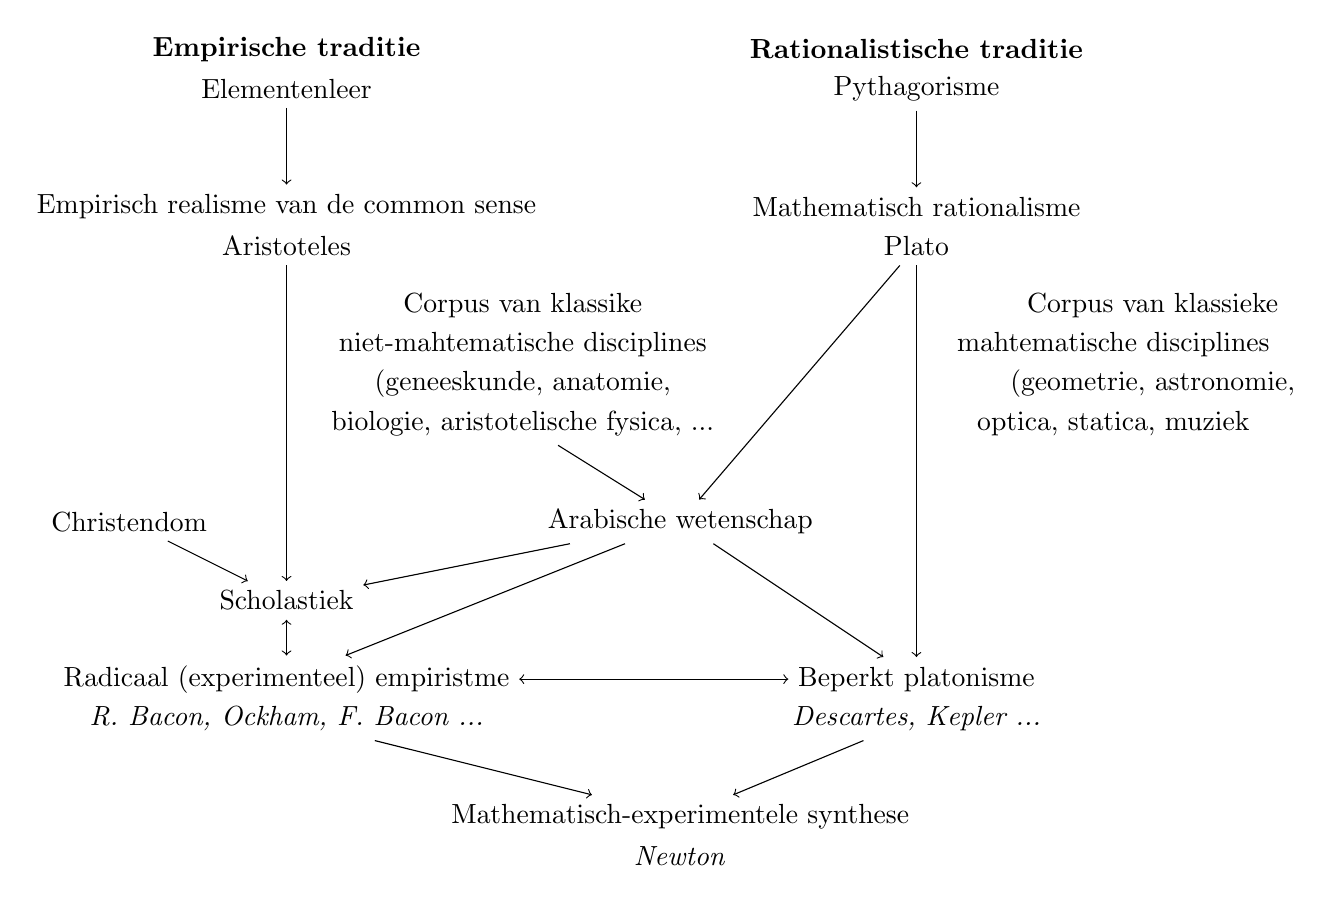
\begin{tikzpicture}
\node (a1) at (-20,0) {\textbf{Empirische traditie}};
\node (a2) at (-12,0) {\textbf{Rationalistische traditie}};
\node (b1) at (-20,-0.5) {Elementenleer};
\node (b2) at (-12,-0.5) {Pythagorisme};
\node (c1) at (-20, -2) {Empirisch realisme van de common sense};
\node (c2) at (-12, -2) {Mathematisch rationalisme};
\node (d1) at (-20,-2.5) {Aristoteles};
\node (d2) at (-12, -2.5) {Plato};

\node (et1) at (-17,-3.25) {Corpus van klassike};
\node (et2) at (-17,-3.75) {niet-mahtematische disciplines};
\node (et3) at (-17,-4.25) {(geneeskunde, anatomie,};
\node (et4) at (-17,-4.75) {biologie, aristotelische fysica, ...};

\node (ft1) at (-9,-3.25) {Corpus van klassieke};
\node (ft2) at (-9.5,-3.75) {mahtematische disciplines};
\node (ft3) at (-9,-4.25) {(geometrie, astronomie,};
\node (ft4) at (-9.5,-4.75) {optica, statica, muziek};

\node (g1) at (-22, -6){Christendom};
\node (g2) at (-15, -6){Arabische wetenschap};

\node (h) at (-20,-7){Scholastiek};
\node (i1) at (-20, -8){Radicaal (experimenteel) empiristme};
\node (i2) at (-12, -8){Beperkt platonisme};

\node (j1) at (-20, -8.5) {\textit{R. Bacon, Ockham, F. Bacon ...}};
\node (j2) at (-12, -8.5) {\textit{Descartes, Kepler ...}};

\node (k) at (-15, -9.75) {Mathematisch-experimentele synthese};
\node (l) at (-15, -10.25) {\textit{Newton}};


\path
(b1) edge[->] (c1)
(b2) edge[->] (c2)
(d1) edge[->] (h)
(d2) edge[->] (i2)
(d2) edge[->] (g2)
(et4) edge[->] (g2)
(g1) edge[->] (h)
(g2) edge[->] (h)
(g2) edge[->] (i1)
(g2) edge[->] (i2)
(h) edge[<->] (i1)
(i2) edge[<->] (i1)
(j1) edge[->] (k)
(j2) edge[->] (k);
\end{tikzpicture}
\end{figure}

\begin{itemize}

\item De enkelvoudige pijlen stellen lijnen van be\"invloeding voor, de dubbele pijlen tegenstellingen (die soms ook verwantschap insluiten).
\item Beide grote lijnen zijn onderweg van buitenaf be\"invloed, door christendom en Arabische wetenschap en filosofie (en de traditie van de magi).
\end{itemize}

\section{Kritiek en constructie}
\subsection{Een dubbelzinnig scepticus?}
HUME neemt de empiristische erfenis van de BACONs over en werkt die uit tot een even indrukwekkende filosofie als die van de rationalisten, maar totaal anders ge\"orienteerd.
\\
Nooit iets meer dan de waarschijnlijkheid kunnen bereiken.
\\
Herhaling en gewoonte  oorzaak en gevolg. Zeker zijn van twijfel. 
\\
HUME wil ons bevrijden van de zoektocht naar onze schijnzekerheden.
\\
\\
Slotsom: Kennis is een bouwsel opgetrokken van op de ervaring, en de beste theorieën die we daaruit induceren zijn waarschijnlijke hypothesen. 
\\
\\
\textbf{Drie putnen van twijfel, drie praktische zekerheden:}

\begin{enumerate}
\item \textbf{Causaliteit:} 
\begin{itemize}
\item Niet meer dan de vaste opeenvolging van fenomeen A en fenomeen B in de waarneming: een gewoont (associate), dus subjectief.
\item Een natural belief.
\end{itemize}

\item \textbf{Inductieprobleem:}
\begin{itemize}
\item Logische sprong; einde van de zekerheid; oplossing: geen radicaal maar gematigd scepticisme; overgang naar waarschijnlijkheid.
\item Een natural belief.
\end{itemize}

\item \textbf{Personal identity}
\begin{itemize}
\item Een constructie, er is alleen een $+/-$ continue bewustzijnstroom
\item Een natural belief: \begin{itemize}
\item Sociaal: we maken elkaar in de omgang tot vaste personen.
\item Criterium van lichamelijke continu\"iteit doorheen tijd en ruimte.
\end{itemize}
\end{itemize}
\end{enumerate}
\subsection{De onverbiddelijke verzoener}
Niet te kennen!
\subsection{Kantiaans constructivisme}
Niet te kennen!
\subsection{... en de zin van alles?}
Niet te kennen!
\section{Positivisten en popperianen}
Niet te kennen!
